\chapter{Evaluation}

In order to investigate the dynamic behavior of the simulation, we must first calibrate the system by choosing our parameters. Most parameters have been inspired by the AppEco experiment which itself uses Apple's App Store chronological data for the callibration.

\section{Calibration}

The parameters used for simulation are shown in Section~\ref{list:simulation_params}. The growth of developers, users, services and devices are shown in Figure~\ref{fig:growth_dev_user_services}.

\begin{figure}[!htb]
  \centering
  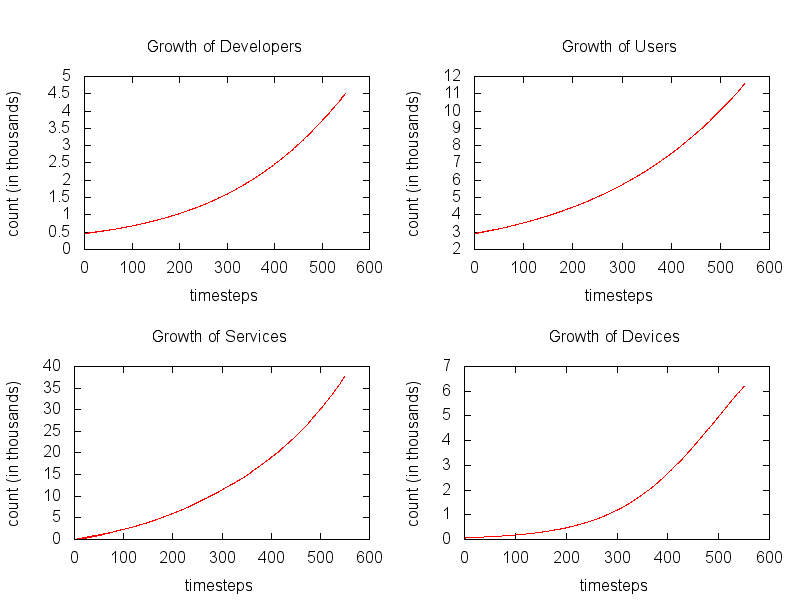
\includegraphics[width=14cm]{figures/dev_user_service_device.png}
  \caption{Growth of developers, users, services and devices over time}
  \label{fig:growth_dev_user_services}
\end{figure}

Growth of population for users and developers are a part of sigmoid growth as explained in Eq.~\ref{eq:s2eco_algorithm}. The growth of services increases exponentially over time. This is because as the population increases, the number of active developers per day increases producing more services. The growth of developers also follow a sigmoid curve but with different parameters. The assumption is at the start of the simulation, developers are interested in less number of devices. As time increases, the variety of devices that developers are interested also increase.

We run the simulation for around 550 timesteps (550 days).

\section{Implementation}

The simulation was coded in Ruby and the graphs were drawn using Gnuplot. Ruby is not as fast as C and C++ but was chosen due to author's familiarity with the language. The simulation takes significant amount of processing time (one day to simulate 100,000 developers and 400,000 users). The simulation is thus broken down into two parts:

\begin{itemize}
  \item User vote simulation. This simulation is focussed on observing feedback of users on services.
  \item Context model convergence simulation: This simulation is focussed on how context models are reused by developers and how they form their network.
\end{itemize}

\section{Experiments}
\label{sec:experiments}

\subsection{User vote simulation for service convergence}

\textbf{Q} How does user feedback affect the services?

To answer the question, we ran the simulation for 550 timesteps (equivalent to 550 days). For each category of developers: \emph{Improvers}, \emph{Ignorers} and \emph{Malicious}; we observed the average rating of the services uploaded to the S2Store. The following graph as shown in Figure~\ref{fig:votes_distribution_segregated} was observed.

\begin{figure}[!htb]
  \centering
  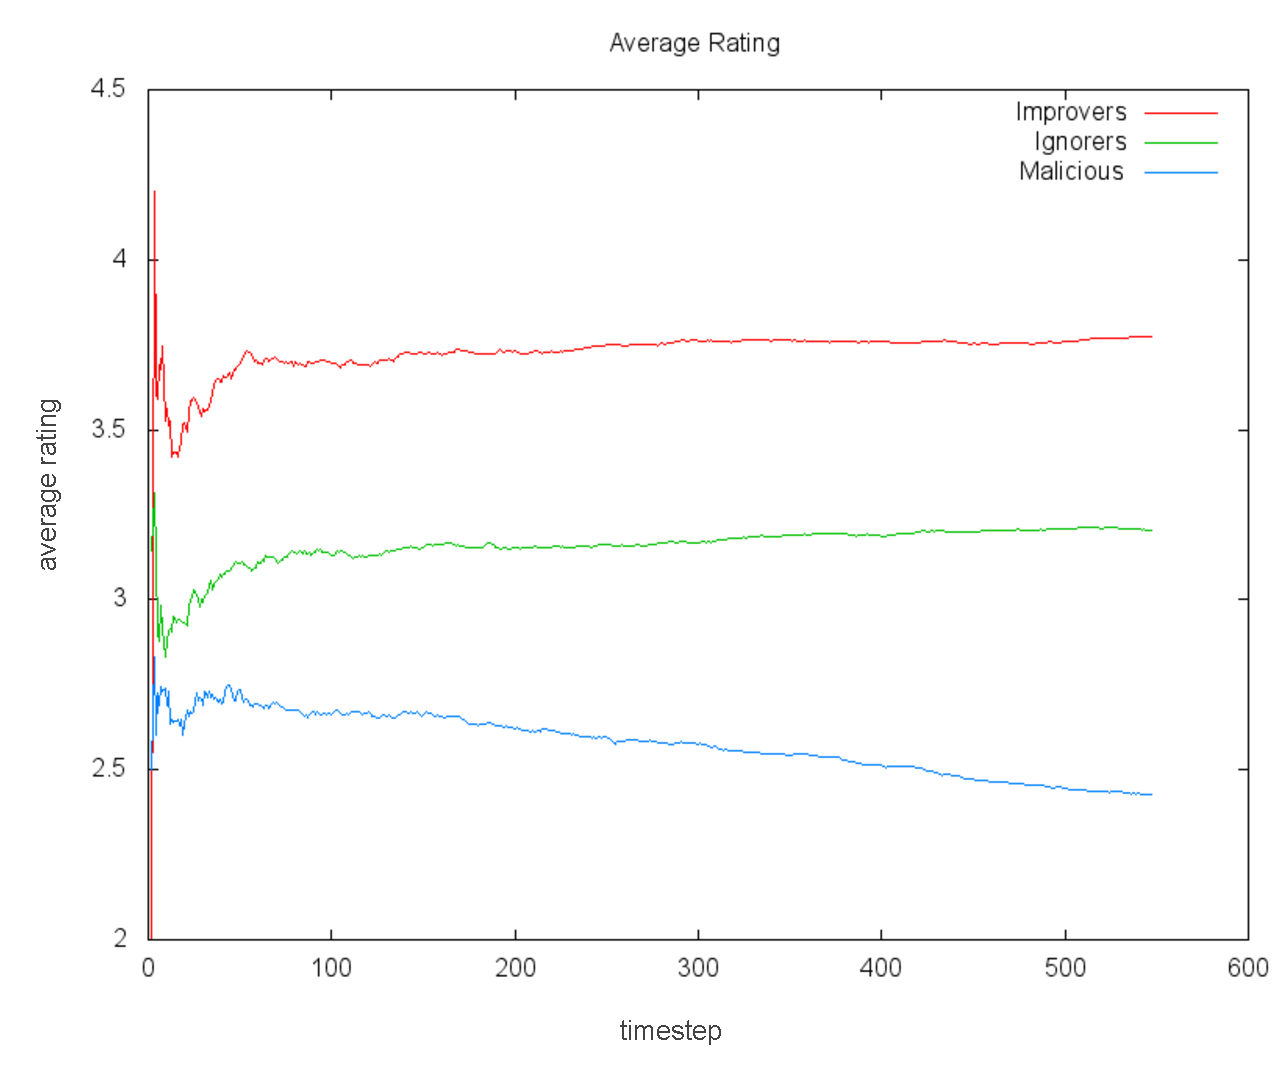
\includegraphics[width=13.5cm]{figures/votes_distribution_segregated.pdf}
  \caption{Distribution of votes among among Improvers, Ignorers and Malicious Developers}
  \label{fig:votes_distribution_segregated}
\end{figure}

Figure~\ref{fig:votes_distribution_segregated}, shows the average vote received under each category of developers. The red line shows the average vote for \emph{Improvers}, the green line shows the average vote for \emph{Ignorers} and the blue line shows the average vote for \emph{Malicious} developers.

The average vote for \emph{Improvers} stay around 3.75 out of 5 and increases gradually. While the average vote of \emph{Ignorers} also stay around 3.2 out of 5, the ratings for \emph{Malicious} users decrease gradually over time.

From this Figure~\ref{fig:votes_distribution_segregated}, we can interpret that a developer who is constantly improving the quality of her app is liked by the users more. Users are happy to see bugs fixed in the applications they use. 

Surprisingly for \emph{Ignorers} the average rating did not decrease as expected. We believe the reason for this behavior is that in S2Eco, all services are equally likely to receive votes between 1 and 5. Since \emph{Ignorers} choose not to change anything, the average rating stays around 3.

Unsurprisingly for \emph{Malicious} developers, users quickly discover the presence of bugs of malicious contents and rate them either 1 or 2. Hence the overall average rating of the services fall down gradually.

\begin{figure}[!htb]
  \centering
  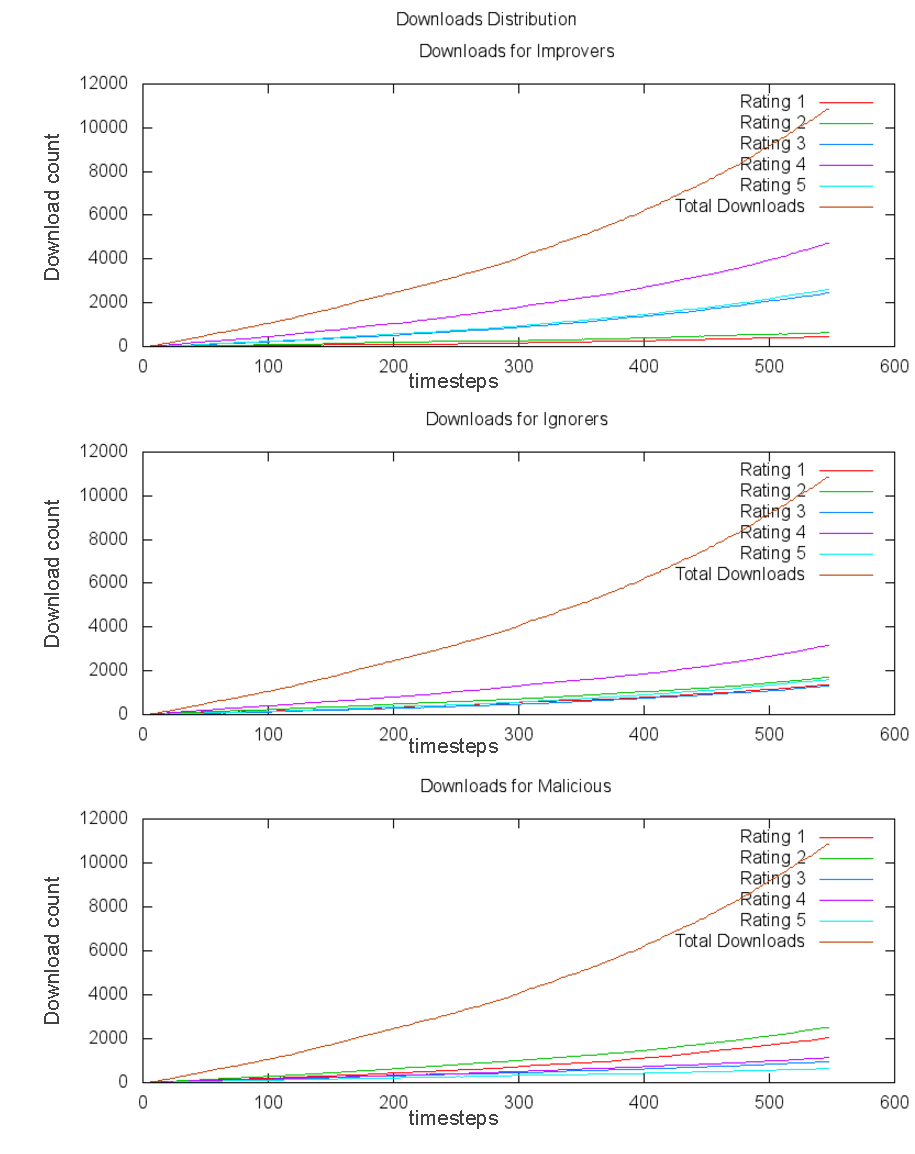
\includegraphics[width=13.5cm]{figures/plot_downloads_segregated.pdf}
  \caption{Distribution of votes among among Improvers, Ignorers and Malicious Developers}
  \label{fig:plot_downloads_segregated}
\end{figure}

From the graph in Figure: \ref{fig:plot_downloads_segregated}, we see that the total number of downloads received by services developed by all three categories remain the same. This is shown by the red top most line in all three graphs. The reason why different categories did not receive different download counts was because in current simulation, users decision to download a service is not influenced by existing rating of that service. User only provides a feedback into the system once she has downloaded and installed the service.

Since \emph{Improvers} constantly improve their services, in long term the users using these services have better experience compared to other categories. This is seen from the first graph where for \emph{Improvers}, most downloaded services have an average rating of 4 while services with 1 and 2 ratings are least downloaded. In contrast in second and third graphs, services with any ratings are equally downloaded.

\subsection{Developer and device interaction simulation for context model convergence}

\textbf{Q} How does developer behave with different information from S2Store and how it affect context model convergence?

To answer the question, we look at the graph shown in Figure: \ref{fig:result_component_relationship}. The three connected cliques are related to three devices (red circle). Each of the devices are connected with three, one and two context models (green) and each of these context models are connected with services (blue circle).

\begin{figure}[!htb]
  \centering
  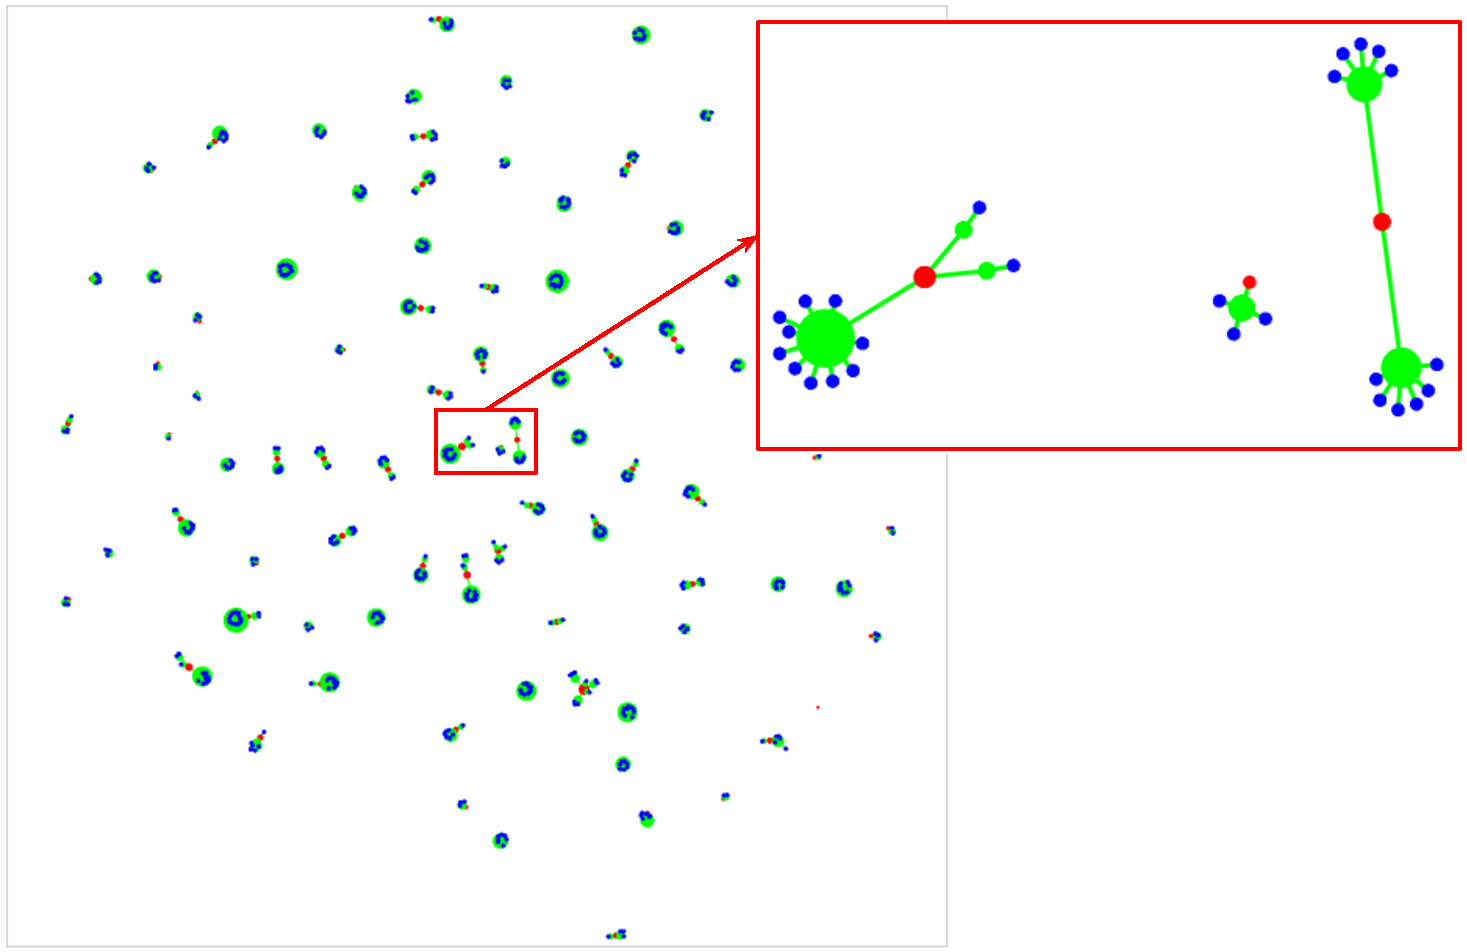
\includegraphics[width=13cm]{figures/result_component_relationship.pdf}
  \caption{Inter-relationship between devices (red), context models (green) and services (blue) at timestep = 25 days}
  \label{fig:result_component_relationship}
\end{figure}

At the beginning of the simulation, S2Eco only produces services that are likely to have only one context model and thus only one device. However, different services can refer to the same device, with different context models. In the figure, the size of the context models (green circle) shows the number of attached services to it.

\begin{figure}[!htb]
  \centering
  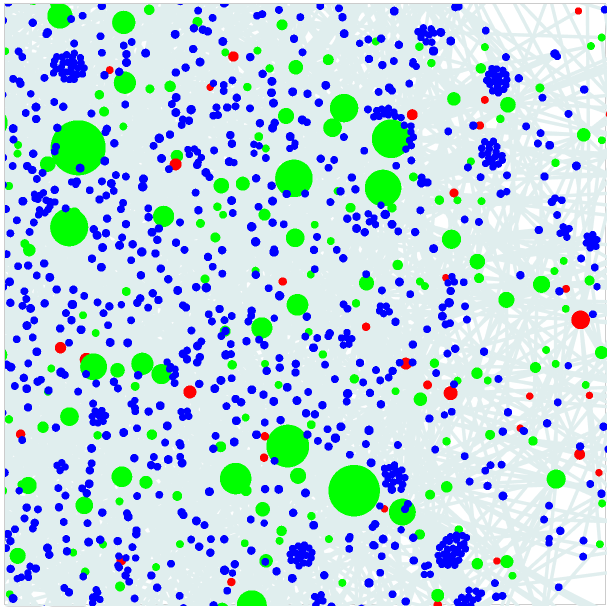
\includegraphics[width=9cm]{figures/result_component_relationship_99.png}
  \caption{Inter-relationship between devices (red), context models (green) and services (blue) at timestep = 99 days}
  \label{fig:result_component_relationship_99}
\end{figure}

After 99 timesteps, the graph was seen as in Figure: \ref{fig:result_component_relationship_99}. The edges have been removed to make the image more clear. It can be seen that more popular context models (larger green circles) have more services (blue circle) around its periphery. Smaller context models have less services around their periphery. The trend increases as the simulation progresses.

\begin{figure}[!htb]
  \centering
  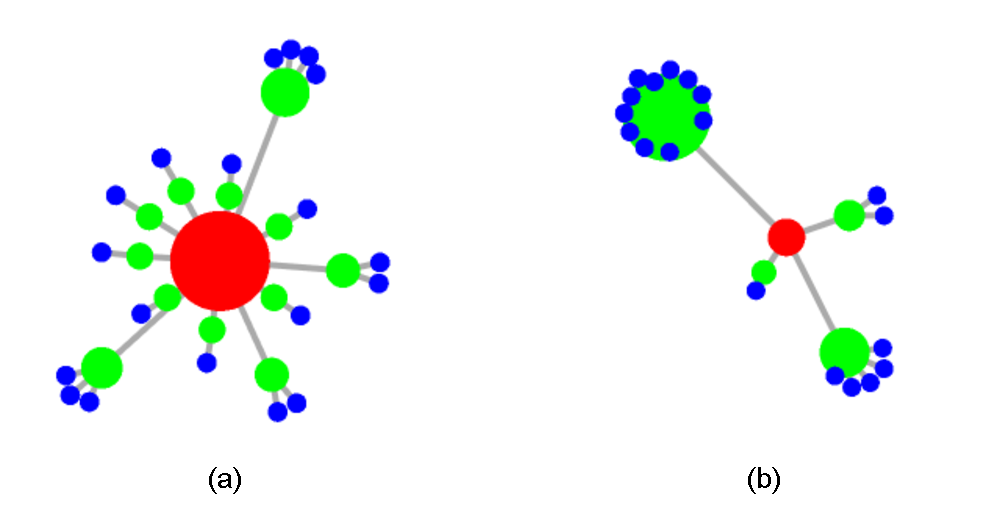
\includegraphics[width=9cm]{figures/result_compare_graph_user_personality.pdf}
  \caption{Two graphs resulting from two different experiments. Graph on the left (a) has a device at the center (red) with many context models associated with it. The context models are almost equal is their degree centrality. There is no clear favorite here. Graph on the right (b) has less context model and one context model is a clear favorite with many services attached to it.}
  \label{fig:result_compare_graph_user_personality}
\end{figure}

It is important for S2Store to be able to provide information about existing context models and their statistics to the developers. A developer is more likely to reuse existing context model when she finds the detail she is looking for. To see how this affects the production of context models, we simulate it in S2Eco. There are two different experiments associated with the graphs in Figure: \ref{fig:result_compare_graph_user_personality}. In the first experiment, developers  had less information. So they had equal probability to either choose existing context model or create a new one themselves. In the second experiment, developers had more information. So the chance that they would select existing context model to creating a new one was $10:1$.

In the first experiment, developers contribute duplicate context models to the store. There are more context models per device with each service using its own context model. Thus, they are not portable with eachother.

In the second experiment, there are less context models per device. One context model is a clear favorite among the developers as they contribute more services to it than other context models. The group of services that are dependent on the same context model are compatible and take benefit from eachother.
